\documentclass[letterpaper, 11pt]{report}
\usepackage{titlesec}
\usepackage{fullpage} % changes the margin
\usepackage{amsmath}
\usepackage{amssymb}
\usepackage{graphicx} %package to manage images
\usepackage[linkcolor=red]{hyperref}
\usepackage{paralist}
\usepackage{subcaption}
\graphicspath{ {./images/} }
\setlength\parindent{0pt}
\begin{document}
\begin{titlepage}
\vspace*{0.7in}
\begin{center}
\begin{figure}[htb]
\begin{center}

\includegraphics[width=8cm]{univ_logo}
\end{center}
\end{figure}
\vspace*{0.3in}
\begin{Large}
\textbf{SOEN 6011 : SOFTWARE ENGINEERING PROCESSES} \\
\end{Large}
\vspace*{0.1in}
\begin{Large}
\textbf{SUMMER 2022} \\
\end{Large}
\vspace*{0.9in}
\begin{Large}
\textbf{F2: Tangent Function, $tan(x)$} \\
\end{Large}
\vspace*{0.625in}
\rule{80mm}{0.1mm}\\
\vspace*{0.1in}
\begin{large}
Author \\
\vspace*{0.1in}
Zeyu Huang\\

\vspace*{0.3in}
\date{\normalsize\today} 
\end{large}
\end{center}
\begin{center}
https://www.overleaf.com/project/62cdb1d5b13422add2cceb12\end{center}
\end{titlepage}
\tableofcontents
\newpage
\addcontentsline{toc}{section}{1) Problem 1}
\addcontentsline{toc}{subsection}{a) Description of Function}
\section*{Problem1}
\subsection*{Description of Function}
 \normalsize{ \cite{test1} $tan(x)$  is a periodic function which is very important in trigonometry. The simplest way to understand the tangent function is to use the unit circle. For a given angle measure $\theta$ draw a unit circle on the coordinate plane and draw the angle centered at the origin, with one side as the positive  x -axis. The  x -coordinate of the point where the other side of the angle intersects the circle is $cos(θ)$ and the  y -coordinate is $sin(θ)$. So, the tangent function is define as below: \[tan(x) = \frac{sin(x)}{cos(x)}\]\\}
The below graph shows values corresponding to different angles.
 \begin{center}
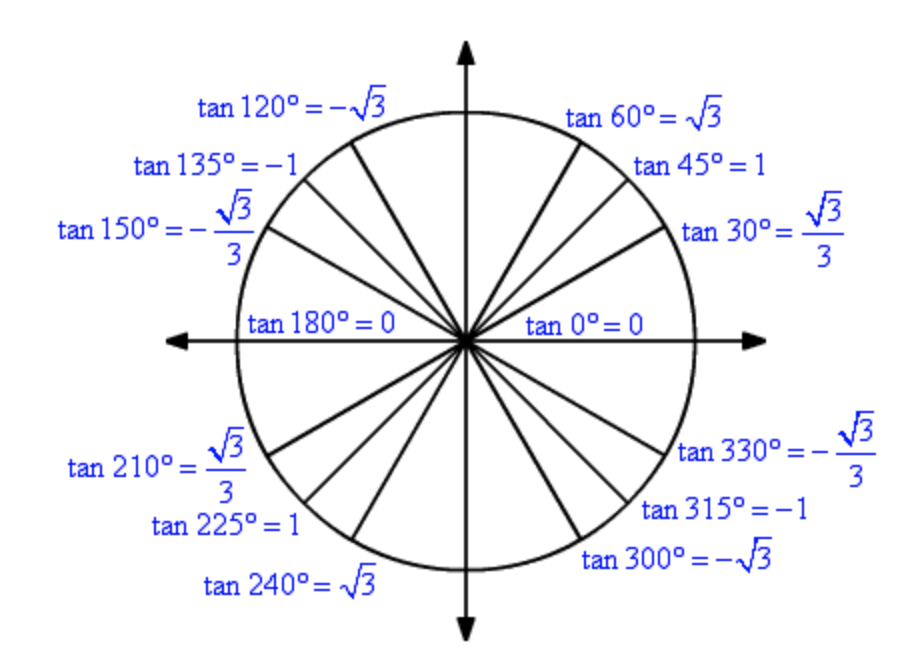
\includegraphics[width= 6cm]{images/tan3.png}
\end{center}
 \\
 \normalsize{ \cite{test1}\cite{varsitytutors}The tangent function is undefined when $x$ $=$ $\pi$ / 2 $+$ $n \pi$ (where, $n$ is integer) for which, $cos(x) = 0$. However, Tangent function does not have an amplitude. In addition, The graph intercept $x$-axis at $n\pi$ (where $n$ is integer) and in $y$-axis at $(0,0)$ point. The period of tangent function is $\pi$.
 }
 \\
 \subsection*{Range}\cite{test1}\cite{varsitytutors}
 \normalsize{ The range of $tan(x)$ is all real number $\mathbb{R}$, $(- \infty, + \infty)$. }
 
 \subsection*{Domain and Co-domain}\cite{test1}\cite{varsitytutors}
 \normalsize{The domain of tangent function is $x \in$ $\mathbb{R}$, $x$ $\neq$ $\pi$ / 2 $+$ $n \pi$ where, $n$ is an integer. The co-domain of $tan(x)$ is \((-\infty, +\infty\)).}

\pagebreak
\newpage
\addcontentsline{toc}{subsection}{b) Context of Use Model}
\section*{Context of Use Model}
\normalsize{Users can use the calculator to calculate the result of $sin()$, $cos()$ and $\frac{sin()}{cos()}$ which is $tan()$ of a degree. This degree shall be an integer or decimal, so the digits \textit{0-9} and the decimal point must be available by the user. The user can select the appropriate function they want to use, and they shall be able to press a button to have the answer computed. The calculator should return the result or an error message that indicates why it was unable to do so.}
\begin{center}
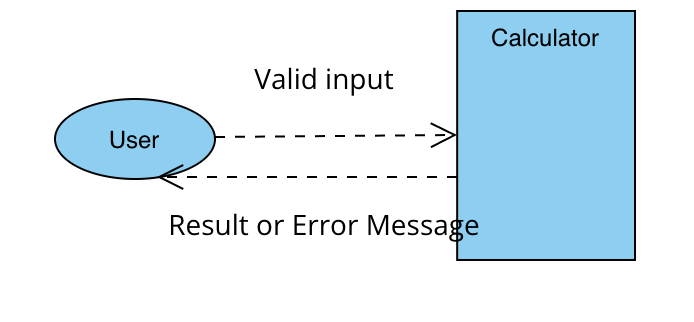
\includegraphics[width=15cm]{context_diagram}
\end{center}
\pagebreak
\newpage
\addcontentsline{toc}{section}{2) Problem 2}
\section*{Problem 2}
\subsection*{Assumption:} 
 For the given degree x, return the result of $tan(x)$. If the input value is invalid or cannot be calculated, return an error message.

\\
\subsection*{Requirements:} \\
\begin{tabular}{ |c|c| } 
 \hline
 \textbf{Requirement Id} & R1 \\ 
   \hline
 \textbf{Overview} & $x = 0^\circ $ + $n\pi$  \\
  \hline
  \textbf{Description} & 
\begin{tabular}[c]{@{}l@{}} For the given input $x = 0^\circ $ ,
the function \\may return 0 as output.
\end{tabular} \\
  \hline
\textbf{Priority} & High \\ 
  \hline
\textbf{Type} & Functional \\
  \hline
\textbf{Difficulty} & Easy \\
  \hline
\end{tabular}

\bigskip

\begin{tabular}{ |c|c|  } 
 \hline
 \textbf{Requirement Id} & R2 \\ 
   \hline
 \textbf{Overview} &  x is Positive Degree  \\
  \hline
  \textbf{Description} & 
\begin{tabular}[c]{@{}l@{}} For the given input x = any Positive Degree  ,\\
the function may return corresponding\\ $tan(x)$ value as output.
\end{tabular} \\
  \hline
\textbf{Priority} & High \\ 
  \hline
\textbf{Type} & Functional \\
  \hline
\textbf{Difficulty} & Medium \\
  \hline
\end{tabular}\\
\bigskip
\newline
{\leftskip=0cm\relax
\begin{tabular}{ |c|c|  } 
 \hline
 \textbf{Requirement Id} & R3 \\ 
   \hline
 \textbf{Overview} &  x is Negative  Degree  \\
  \hline
  \textbf{Description} & 
\begin{tabular}[c]{@{}l@{}} For the given input x = any Negative Degree  ,\\
the function may return corresponding\\ $tan(x)$ value as output.
\end{tabular} \\
  \hline
\textbf{Priority} & High \\ 
  \hline
\textbf{Type} & Functional \\
  \hline
\textbf{Difficulty} & Medium \\
  \hline
\end{tabular}\\
\bigskip
\newline
\begin{tabular}{ |c|c| } 
 \hline
 \textbf{Requirement Id} & R4 \\ 
   \hline
 \textbf{Overview} & $x = 90^\circ$ + $n\pi$  \\
  \hline
  \textbf{Description} & 
\begin{tabular}[c]{@{}l@{}} For the given input x ,
the function \\may return "Invalid" as output.
\end{tabular} \\
  \hline
\textbf{Priority} & High \\ 
  \hline
\textbf{Type} & Functional \\
  \hline
\textbf{Difficulty} & Hard \\
  \hline
\end{tabular}

\begin{thebibliography}{}
\bibitem{test1}
Varsity Tutors.
\\https://www.varsitytutors.com/hotmath/hotmath$\_$help/topics/tangent-function

\bibitem{varsitytutors} 
varsitytutors.graphing tangent function. 
\\https://www.varsitytutors.com/hotmath/hotmath$\_$help/topics/graphing-tangent-function

\end{thebibliography}
\end{document}
